% === A05 - Memoria Dinamica ===
% David Alejandro Gonzalez Marquez
% dmarquez@dc.uba.ar / fokerman@gmail.com
% https://github.com/fokerman/Orga2Course

\documentclass[aspectratio=169]{beamer}
% \documentclass[handout]{beamer}

% % % Packages
\usepackage[sfdefault]{AlegreyaSans}
\usepackage{inconsolata}
\usepackage{multicol}
\usepackage{multirow}
\usepackage[spanish]{babel}
\usepackage[utf8]{inputenc}
\usepackage{enumerate}
\usepackage{color}
\usepackage{xcolor}
\usepackage[absolute,overlay]{textpos}
  \setlength{\TPHorizModule}{1mm}
  \setlength{\TPVertModule}{1mm}
\usepackage{framed}
\usepackage{mfirstuc} % para poner en mayusculas la primer letra
\usepackage{xspace} % para crear espacios en comandos 
\usepackage{pbox}
\usepackage{tikz}
\usepackage{mathabx}

% % % Beamer config
\usetheme{Pittsburgh}
\usecolortheme[rgb={1,0.48,0.0}]{structure}
\setbeamercolor{block title}{fg=white,bg=verdeuca}
\xdefinecolor{verdeuca}{rgb}{0.0,0.48,0.54}
\xdefinecolor{naranjauca}{rgb}{1,0.48,0.0}
\setbeamercolor{palette quaternary}{fg=white,bg=verdeuca}
\setbeamertemplate{title page}[default][colsep=-4bp, rounded=true] % remove title shadow
\setbeamertemplate{frametitle}[default][colsep=-2bp, shadow=false] % remove frame title shadow
\setbeamertemplate{navigation symbols}{} % remove navigation symbols
\beamertemplatenavigationsymbolsempty

% % % Colors
\definecolor{AzulClaro}{rgb}{.31,.506,.741}
\definecolor{Gris}{gray}{0.8}
\definecolor{Celeste}{rgb}{.255,.41,.884}
\definecolor{Rojo}{rgb}{1, 0, 0}

% % % Rename
\newcommand{\tab}[0]{\hspace{15pt}}

% % % Blocks
\setbeamercolor{block body}{fg=black, bg=black!10}
\setbeamercolor{block title}{fg=black, bg=black!20}
\setbeamercolor{coloredboxstuffNaranja}{fg=naranjauca,bg=black!10} %% PARA LOS BOX
\setbeamercolor{coloredboxstuffVerde}{fg=verdeuca,bg=black!10} %% PARA LOS BOX

% % % Start

\title{\Huge Memoria Dinámica}
\subtitle{Estructuras, Malloc/Free y Listas}
\author{David Alejandro González Márquez}
\institute{Departamento de Computación\\
Facultad de Ciencias Exactas y Naturales\\
Universidad de Buenos Aires}
\date{}

\begin{document}

\begin{frame}[plain]
    \titlepage 
\end{frame}

\begin{frame}[fragile]
    \frametitle{Hoy}
    \LARGE
    \begin{itemize}
    \item Estructuras
    \vspace{1cm}
    \item Memoria Dinámica
    \vspace{1cm}
    \item Listas
    \vspace{1cm}
    \item Ejercicios
    \end{itemize}
\end{frame}

\begin{frame}[fragile]
    \frametitle{Estructuras}
    \large
    \begin{itemize}
     \item[-] Definen un \textbf{patrón de acceso} a memoria.
     \begin{itemize}
     \item[-] \normalsize Equivalente a un esténcil para nombrar a un conjunto de bytes.
     \end{itemize}
     \pause
     \vspace{0.3cm}
     \item[-] Se declaran como una \textbf{lista de campos} con su nombre y tipo.
     \begin{itemize}
     \item[-] \normalsize Desde ASM debemos conocer los tamaños de cada uno,
     \item[-] \normalsize y calcular el \texttt{offset} en bytes a cada campo.
     \end{itemize}
     \pause
     \vspace{0.3cm}
     \item[-] Los structs pueden ser:
     \begin{itemize}
     \item[-] \normalsize \texttt{packed}: No respeta reglas de alineación.
     \item[-] \normalsize \texttt{unpacked}: Respeta reglas de alineación.
     \end{itemize}
    \end{itemize}

\end{frame}

\begin{frame}[fragile]
    \frametitle{Estructuras}
    \begin{block}{\texttt{struct}}
    Definen un patrón de acceso a un área determinada de memoria\\
    \vspace{0.2cm}
    \hspace{2cm} \texttt{struct} \textcolor{naranjauca}{\textit{nombre\_de\_la\_estructura}} \texttt{\{}\\
    \hspace{2cm} \hspace{2cm} \textcolor{naranjauca}{\textit{tipo\_1}} \hspace{0.5cm} \textcolor{naranjauca}{\textit{nombre\_del\_campo\_1}} \texttt{;}\\
    \hspace{2cm} \hspace{2cm} \texttt{...}\\
    \hspace{2cm} \hspace{2cm} \textcolor{naranjauca}{\textit{tipo\_n}} \hspace{0.5cm} \textcolor{naranjauca}{\textit{nombre\_del\_campo\_n}} \texttt{;}\\
    \hspace{2cm} \texttt{\}}\\
    \end{block}
    \uncover<2->{Ejemplos:} \uncover<3->{\textcolor{verdeuca}{$\rightarrow$ \texttt{SIZE}}} \uncover<4->{\textcolor{verdeuca}{$\Rightarrow$ \texttt{OFFSET}}}\\
    \begin{multicols}{2}
    \begin{tabular}{lll}
    \uncover<2->{\texttt{struct p2D \{}} & \\
    \uncover<2->{\texttt{      int x;}}  & \uncover<3->{\textcolor{verdeuca}{$\rightarrow 4$}} & \uncover<4->{\textcolor{verdeuca}{$\Rightarrow 0$}}\\
    \uncover<2->{\texttt{      int y;}}  & \uncover<3->{\textcolor{verdeuca}{$\rightarrow 4$}} & \uncover<4->{\textcolor{verdeuca}{$\Rightarrow 4$}}\\
    \uncover<2->{\texttt{\};}}           &                                                     & \uncover<4->{\textcolor{verdeuca}{$\Rightarrow 8$}}\\
    \end{tabular}
    \columnbreak
    \begin{tabular}{lll}
    \uncover<5->{\texttt{struct alumno \{}}     & &\\
    \uncover<5->{\texttt{      char* nombre;}}  & \uncover<6->{\textcolor{verdeuca}{$\rightarrow 8$}} & \uncover<7->{\textcolor{verdeuca}{$\Rightarrow 0$}}\\
    \uncover<5->{\texttt{      char comision;}} & \uncover<6->{\textcolor{verdeuca}{$\rightarrow 1$}} & \uncover<8->{\textcolor{verdeuca}{$\Rightarrow 8$}}\\
    \uncover<5->{\texttt{      int dni;}}       & \uncover<6->{\textcolor{verdeuca}{$\rightarrow 4$}} & \uncover<9->{\textcolor{verdeuca}{$\Rightarrow 12$}}\\
    \uncover<5->{\texttt{\};}}                  &                                                     & \uncover<10->{\textcolor{verdeuca}{$\Rightarrow 16$}}\\
    \end{tabular}
    \end{multicols}
\end{frame}

\begin{frame}
    \frametitle{Alineación}
    \begin{itemize}
    \item \textcolor{verdeuca}{Alineación en los campos del struct:}\\
    Cada campo esta alineado a su tamaño dentro del struct
    \begin{center}
    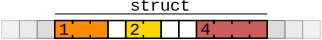
\includegraphics[scale=0.7]{img/struct_aling.pdf}
    \end{center}
    \vspace{0.5cm} \pause
    \item \textcolor{verdeuca}{Tamaño del struct:}\\
    Debe ser múltiplo del campo más grande del struct
    \begin{center}
    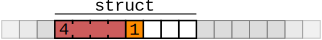
\includegraphics[scale=0.7]{img/struct_total_size.pdf}
    \end{center}
    \vspace{0.5cm} \pause
    \item \textcolor{verdeuca}{\texttt{\_\_attribute\_\_((packed))}:}\\
    Indica que el struct no va a ser alinenado
    \begin{center}
    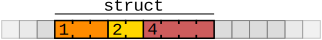
\includegraphics[scale=0.7]{img/struct_packet.pdf}
    \end{center}
    \end{itemize}
\end{frame}

\begin{frame}[fragile]
    \frametitle{Ejemplos}
    \begin{textblock}{100}(10,10)
    \frametitle{Ejemplos: \hspace{3.3cm} \uncover<2->{$\rightarrow$ \texttt{SIZE}} \uncover<4->{$\Rightarrow$ \texttt{OFFSET}} }
    \hspace{1cm}
    \begin{tabular}{lll}
    \texttt{struct alumno \{}   & & \\
    \texttt{    char* nombre;}  & \uncover<2->{\textcolor{verdeuca}{$\rightarrow 8$}} & \uncover<4->{\textcolor{verdeuca}{$\Rightarrow 0$}}\\
    \texttt{    char comision;} & \uncover<2->{\textcolor{verdeuca}{$\rightarrow 1$}} & \uncover<5->{\textcolor{verdeuca}{$\Rightarrow 8$}}\\
    \texttt{    int dni;}       & \uncover<2->{\textcolor{verdeuca}{$\rightarrow 4$}} & \uncover<6->{\textcolor{verdeuca}{$\Rightarrow 12$}}\\
    \texttt{\};}                &                                                     & \uncover<7->{\textcolor{verdeuca}{$\Rightarrow 16$}} \vspace{0.3cm}\\
    \texttt{struct alumno2 \{}  & & \\
    \texttt{    char comision;} & \uncover<2->{\textcolor{verdeuca}{$\rightarrow 1$}} & \uncover<8->{\textcolor{verdeuca}{$\Rightarrow 0$}}\\
    \texttt{    char* nombre;}  & \uncover<2->{\textcolor{verdeuca}{$\rightarrow 8$}} & \uncover<9->{\textcolor{verdeuca}{$\Rightarrow 8$}}\\
    \texttt{    int dni;}       & \uncover<2->{\textcolor{verdeuca}{$\rightarrow 4$}} & \uncover<10->{\textcolor{verdeuca}{$\Rightarrow 16$}}\\
    \texttt{\};}                &                                                     & \uncover<11->{\textcolor{verdeuca}{$\Rightarrow 24$}} \vspace{0.3cm}\\
    \texttt{struct alumno3 \{}  & & \\
    \texttt{    char* nombre;}  & \uncover<2->{\textcolor{verdeuca}{$\rightarrow 8$}} & \uncover<12->{\textcolor{verdeuca}{$\Rightarrow 0$}}\\
    \texttt{    int dni;}       & \uncover<2->{\textcolor{verdeuca}{$\rightarrow 4$}} & \uncover<13->{\textcolor{verdeuca}{$\Rightarrow 8$}}\\
    \texttt{    char comision;} & \uncover<2->{\textcolor{verdeuca}{$\rightarrow 1$}} & \uncover<14->{\textcolor{verdeuca}{$\Rightarrow 12$}}\\
    \multicolumn{2}{l}{ \texttt{\} \_\_attribute\_\_((packed));} }                    & \uncover<15->{\textcolor{verdeuca}{$\Rightarrow 13$}}\\
    \end{tabular}
    \end{textblock}

    \begin{textblock}{50}(100,9.2) \only<3->{\includegraphics[scale=0.7]{img/struct_814-layer1.pdf}} \end{textblock}
    \begin{textblock}{50}(100,9.2) \only<4->{\includegraphics[scale=0.7]{img/struct_814-layer2.pdf}} \end{textblock}
    \begin{textblock}{50}(100,9.2) \only<5->{\includegraphics[scale=0.7]{img/struct_814-layer3.pdf}} \end{textblock}
    \begin{textblock}{50}(100,9.2) \only<6->{\includegraphics[scale=0.7]{img/struct_814-layer4.pdf}} \end{textblock}
    \begin{textblock}{50}(100,9.2) \only<7->{\includegraphics[scale=0.7]{img/struct_814-layer5.pdf}} \end{textblock}

    \begin{textblock}{50}(100,36.1) \only<3->{\includegraphics[scale=0.7]{img/struct_184-layer1.pdf}} \end{textblock}
    \begin{textblock}{50}(100,36.1) \only<8->{\includegraphics[scale=0.7]{img/struct_184-layer2.pdf}} \end{textblock}
    \begin{textblock}{50}(100,36.1) \only<9->{\includegraphics[scale=0.7]{img/struct_184-layer3.pdf}} \end{textblock}
    \begin{textblock}{50}(100,36.1) \only<10->{\includegraphics[scale=0.7]{img/struct_184-layer4.pdf}} \end{textblock}
    \begin{textblock}{50}(100,36.1) \only<11->{\includegraphics[scale=0.7]{img/struct_184-layer5.pdf}} \end{textblock}
    
    \begin{textblock}{50}(100,63) \only<3->{\includegraphics[scale=0.7]{img/struct_841-layer1.pdf}} \end{textblock}
    \begin{textblock}{50}(100,63) \only<12->{\includegraphics[scale=0.7]{img/struct_841-layer2.pdf}} \end{textblock}
    \begin{textblock}{50}(100,63) \only<13->{\includegraphics[scale=0.7]{img/struct_841-layer3.pdf}} \end{textblock}
    \begin{textblock}{50}(100,63) \only<14->{\includegraphics[scale=0.7]{img/struct_841-layer4.pdf}} \end{textblock}
    \begin{textblock}{50}(100,63) \only<15->{\includegraphics[scale=0.7]{img/struct_841-layer5.pdf}} \end{textblock}

\end{frame}

\begin{frame}[fragile,t]
    \frametitle{Uso}
    \begin{textblock}{50}(30,10)
        \only<2->{
        \begin{tabular}{ll}
        \textcolor{verdeuca}{Definición:} \hspace{0.5cm} & \texttt{struct alumno \{}\\
        & \hspace{1cm} \texttt{char* nombre;}\\
        & \hspace{1cm} \texttt{char comision;}\\
        & \hspace{1cm} \texttt{int dni;}\\
        & \texttt{\};}\\
        \end{tabular}
        }
    \end{textblock}
    \begin{textblock}{50}(20,35)
        \only<3->{
        \textcolor{verdeuca}{Uso en C:}\\
        \vspace{0.2cm}
        \textcolor{naranjauca}{\texttt{struct alumno}} \texttt{ alu1;}\\
        \vspace{0.1cm}
        \texttt{alu1.nombre = \textquotesingle{}carlos\textquotesingle{};}\\
        \texttt{alu1.dni = alu.dni + 10;}\\
        \texttt{alu1.comision = \textquotesingle{}a\textquotesingle{};}\\
        \vspace{0.2cm}
        }
        \only<4->{
        \textcolor{naranjauca}{\texttt{struct alumno}} \texttt{ *alu2;}\\
        \vspace{0.1cm}
        \texttt{alu2->nombre = \textquotesingle{}carlos\textquotesingle{};}\\
        \texttt{alu2->dni = alu.dni + 10;}\\
        \texttt{alu2->comision = \textquotesingle{}a\textquotesingle{};}        
        }
    \end{textblock}
    \begin{textblock}{50}(80,35)
        \only<5->{
        \textcolor{verdeuca}{Uso en ASM:}\\
        \vspace{0.2cm}
        \texttt{\%define off\_nombre 0}\\
        \texttt{\%define off\_comision 8}\\
        \texttt{\%define off\_dni 12}\\
        \vspace{0.2cm}
        }
        \only<6->{
        \texttt{mov rsi,} \textcolor{naranjauca}{\texttt{ptr\_struct}}\\
        \texttt{mov rbx, [rsi+off\_nombre]}\\
        \texttt{mov al, [rsi+off\_comision]}\\
        \texttt{mov edx, [rsi+off\_dni]}
        }
    \end{textblock}
\end{frame}

\begin{frame}[t]
    \frametitle{Memoria}
    \vspace{0.4cm}
    \uncover<1->{
    \begin{block}{Variable estática}
    Esta asignada en un espacio de memoria reservado que solo será utilizado para almacenar la variable en cuestión.
    \end{block}
    }
    \begin{textblock}{100}(10,40)
    \only<2>{
    \textcolor{naranjauca}{Ejemplo ASM:}\\
    \vspace{0.3cm}
    \begin{tabular}{ll}
                                    & \textcolor{verdeuca}{\texttt{section .data:}} \\
                                    & \hspace{0.5cm}\texttt{   numero: dd 10} \vspace{0.3cm}\\
                                    & \textcolor{verdeuca}{\texttt{section .rodata:}} \\
                                    & \hspace{0.5cm}\texttt{mensaje: db \textquotesingle{}hola pepe\textquotesingle{}} \vspace{0.3cm}\\
                                    & \textcolor{verdeuca}{\texttt{section .bss}} \\
                                    & \hspace{0.5cm}\texttt{otro\_numero: resd 1} \\
    \end{tabular}  
    }
    \end{textblock}
    \begin{textblock}{100}(75,40)
    \only<2>{
    \textcolor{naranjauca}{Ejemplo C:}\\
    \vspace{0.3cm}
    \begin{tabular}{ll}
                                    &\\
                                    & \texttt{const int numero = 10;} \vspace{0.3cm}\\
                                    &\\
                                    & \texttt{const char* mensaje = \textquotesingle{}hola pepe\textquotesingle{};} \vspace{0.3cm}\\
                                    &\\
                                    & \texttt{int otro\_numero;} \\
    \end{tabular}
    }
    \end{textblock}
    \uncover<3->{
    \begin{block}{Variable en la pila}
    Esta asignada dentro del espacio de pila del programa, puede existir solo en el contexto de ejecución de una función.
    \end{block}
    }
    \begin{textblock}{100}(20,55)
    \only<4>{
    \begin{tabular}{ll}
             & \\
    ej. ASM: & \texttt{add rbp, 8} \hspace{0.5cm} \textcolor{verdeuca}{\small (Suponer \texttt{rbp} como la base del \emph{stack frame})}\\
             & \\
    ej. C:   & \texttt{int* numero;}\\
    \end{tabular}
    }
    \end{textblock}
    \uncover<5->{
    \begin{block}{Variable dinámica}
    Esta asignada en un espacio de memoria solicitado al sistema operativo mediante una biblioteca de funciones, estas permiten solicitar y liberar memoria. (\texttt{malloc})
    \end{block}
    }
\end{frame}

\begin{frame}
    \frametitle{Memoria}
    \begin{textblock}{100}(7,14) \only<1->{\includegraphics[scale=0.9]{img/memory-layer1.pdf}} \end{textblock}
    \begin{textblock}{100}(7,14) \only<2-4>{\includegraphics[scale=0.9]{img/memory-layer2.pdf}} \end{textblock}
    \begin{textblock}{100}(7,14) \only<2->{\includegraphics[scale=0.9]{img/memory-layer3.pdf}} \end{textblock}
    \begin{textblock}{100}(7,14) \only<3-4>{\includegraphics[scale=0.9]{img/memory-layer4.pdf}} \end{textblock}
    \begin{textblock}{100}(7,14) \only<3->{\includegraphics[scale=0.9]{img/memory-layer5.pdf}} \end{textblock}
    \begin{textblock}{100}(7,14) \only<4-4>{\includegraphics[scale=0.9]{img/memory-layer6.pdf}} \end{textblock}
    \begin{textblock}{100}(7,14) \only<4->{\includegraphics[scale=0.9]{img/memory-layer7.pdf}} \end{textblock}
    \begin{textblock}{100}(7,14) \only<5->{\includegraphics[scale=0.9]{img/memory-layer8.pdf}} \end{textblock}
    \begin{textblock}{100}(7,14) \only<7->{\includegraphics[scale=0.9]{img/memory-layer9.pdf}} \end{textblock}
    \begin{textblock}{100}(7,14) \only<6->{\includegraphics[scale=0.9]{img/memory-layer10.pdf}} \end{textblock}
    \begin{textblock}{100}(7,14) \only<8->{\includegraphics[scale=0.9]{img/memory-layer11.pdf}} \end{textblock}
    \begin{textblock}{100}(7,14) \only<9->{\includegraphics[scale=0.9]{img/memory-layer12.pdf}} \end{textblock}
    \begin{textblock}{100}(7,14) \only<5->{\includegraphics[scale=0.9]{img/memory-layer13.pdf}} \end{textblock}
\end{frame}

\begin{frame}[t]
    \frametitle{Memoria Dinámica}
    \begin{block}{Solicitar memoria}
    \begin{center}
    \textcolor{verdeuca}{\texttt{void *malloc(size\_t size)}}\\
    \end{center}
    Asigna \texttt{size} bytes de memoria y nos devuelve su posición.
    \end{block}
    \vspace{0.5cm}
    \pause
    \begin{block}{Liberar memoria}
    \begin{center}
    \textcolor{verdeuca}{\texttt{void free(void *pointer)}}\\
    \end{center}
    Libera la memoria en \texttt{pointer}, previamente solicitada por \texttt{malloc}.
    \end{block}
    \pause
    \vspace{0.3cm}
    \begin{center}
    \textit{``With a great power comes a great responsibility''} 
    \end{center}
\end{frame}

\begin{frame}[t]
    \frametitle{Memoria Dinámica}
    \begin{block}{Solicitar memoria desde ASM}
    \begin{tabular}{ll}
    \texttt{mov rdi, 24} & \textcolor{verdeuca}{; solicitamos 24 Bytes de memoria}\\
    \texttt{call malloc} & \textcolor{verdeuca}{; llamamos a \texttt{malloc} que devuelve en \texttt{rax}}\\
                         & \textcolor{verdeuca}{; el puntero a la memoria solicitada}
    \end{tabular}
    \end{block}
    \vspace{0.5cm}
    \pause
    \begin{block}{Liberar memoria desde ASM}
    \begin{tabular}{ll}
    \texttt{mov rdi, rax} & \textcolor{verdeuca}{; \texttt{rdi} contiene el puntero a la memoria}\\
                          & \textcolor{verdeuca}{; entregado por \texttt{malloc} al solicitar memoria}\\
    \texttt{call free}    & \textcolor{verdeuca}{; llamamos a \texttt{free}}
    \end{tabular}
    \end{block}
    \pause
    \vspace{0.3cm}
    \begin{center}
    \textit{``With a great power comes a great responsibility'' \\ \textcolor{red}{(Si, también en ASM)}} 
    \end{center}
\end{frame}

\begin{frame}[fragile,t]
    \frametitle{Memoria Dinámica  \hspace{0.5cm}\huge - IMPORTANTE -}

    \normalsize
    Si se solicita memoria utilizando \texttt{malloc}, se \textbf{DEBE} liberar utilizando \texttt{free}.\\
    Toda memoria que se solicite \textbf{DEBE} ser liberada durante la ejecución del programa.\\
    \vspace{0.3cm}
    \pause
    Caso contrario se \hspace{0.03cm} \huge \textcolor{red}{PIERDE MEMORIA} \\
    \vspace{0.3cm}
    \pause
    \normalsize Para detectar problemas en el uso de la memoria se puede utilizar: \\
    \begin{center}
    \Huge \texttt{Valgrind}\\
    \end{center}
    \pause
    \normalsize \textcolor{verdeuca}{Uso:}\\
    \normalsize \verb|$ valgrind --leak-check=full --show-leak-kinds=all -v ./holamundo|\\
    \vspace{0.2cm}
    \normalsize \textcolor{verdeuca}{Instalación:}\\
    \begin{itemize}
    \item[-] Ubuntu/Debian: \texttt{sudo apt-get install valgrind}
    \item[-] Otros Linux/Mac OS: \url{http://valgrind.org/downloads/current.html}
    \item[-] Windows: \textcolor{naranjauca}{usen Linux}
    \end{itemize}
\end{frame}

\begin{frame}[t]
    \frametitle{Listas}
    Estructuras: \only<2->{\textcolor{verdeuca}{$\rightarrow$ \texttt{SIZE}}} \only<3->{\textcolor{verdeuca}{$\Rightarrow$ \texttt{OFFSET}}}
    \begin{multicols}{2}
    \begin{tabular}{lll}
    \texttt{struct lista \{}      &                                                  & \\
    \texttt{      nodo *primero;} & \only<2->{\textcolor{verdeuca}{$\rightarrow 8$}} & \only<3->{\textcolor{verdeuca}{$\Rightarrow 0$}}\\
    \texttt{\};}                  &                                                  & \only<3->{\textcolor{verdeuca}{$\Rightarrow 8$}}\\
    \end{tabular}
    \columnbreak
    \begin{tabular}{lll}
    \texttt{struct nodo \{}     &                                                  & \\
    \texttt{      int dato;}    & \only<2->{\textcolor{verdeuca}{$\rightarrow 4$}} & \only<3->{\textcolor{verdeuca}{$\Rightarrow 0$}}\\
    \texttt{      nodo *prox;}  & \only<2->{\textcolor{verdeuca}{$\rightarrow 8$}} & \only<3->{\textcolor{verdeuca}{$\Rightarrow 8$}}\\
    \texttt{\};}                &                                                  & \only<3->{\textcolor{verdeuca}{$\Rightarrow 16$}}\\
    \end{tabular}
    \end{multicols}
    \begin{textblock}{100}(30,40) \only<4->{\includegraphics[scale=0.7]{img/lista_enteros-layer1.pdf}} \end{textblock}
    \begin{textblock}{100}(30,40) \only<5->{\includegraphics[scale=0.7]{img/lista_enteros-layer2.pdf}} \end{textblock}
    \begin{textblock}{100}(30,40) \only<6->{\includegraphics[scale=0.7]{img/lista_enteros-layer3.pdf}} \end{textblock}
    \begin{textblock}{100}(30,40) \only<7->{\includegraphics[scale=0.7]{img/lista_enteros-layer4.pdf}} \end{textblock}
    \begin{textblock}{100}(30,40) \only<8->{\includegraphics[scale=0.7]{img/lista_enteros-layer5.pdf}} \end{textblock}
\end{frame}

\begin{frame}[t]
    \frametitle{Listas - Agregar}

    \begin{textblock}{100}(20,5) \only<3->{\includegraphics[scale=0.7]{img/lista_enteros_agregar-layer9.pdf}} \end{textblock}  % p. nuevo
    \begin{textblock}{100}(20,5) \only<4->{\includegraphics[scale=0.7]{img/lista_enteros_agregar-layer7.pdf}} \end{textblock}  % dato
    \begin{textblock}{100}(20,5) \only<5->{\includegraphics[scale=0.7]{img/lista_enteros_agregar-layer11.pdf}} \end{textblock} % p. copia

    \begin{textblock}{100}(20,5) \only<1->{\includegraphics[scale=0.7]{img/lista_enteros_agregar-layer1.pdf}} \end{textblock}  % list
    \begin{textblock}{100}(20,5) \only<1-2>{\includegraphics[scale=0.7]{img/lista_enteros_agregar-layer2.pdf}} \end{textblock}  % arrow
    \begin{textblock}{100}(20,5) \only<2,6>{\includegraphics[scale=0.7]{img/lista_enteros_agregar-layer3.pdf}} \end{textblock}  % malloc flecha
    \begin{textblock}{100}(20,5) \only<2->{\includegraphics[scale=0.7]{img/lista_enteros_agregar-layer4.pdf}} \end{textblock}  % malloc
    \begin{textblock}{100}(20,5) \only<3->{\includegraphics[scale=0.7]{img/lista_enteros_agregar-layer5.pdf}} \end{textblock}  % next nuevo
    
    \begin{textblock}{100}(20,5) \only<3->{\includegraphics[scale=0.7]{img/lista_enteros_agregar-layer10.pdf}} \end{textblock} % p. nuevo
    \begin{textblock}{100}(20,5) \only<4->{\includegraphics[scale=0.7]{img/lista_enteros_agregar-layer8.pdf}} \end{textblock}  % dato gris
    \begin{textblock}{100}(20,5) \only<5->{\includegraphics[scale=0.7]{img/lista_enteros_agregar-layer12.pdf}} \end{textblock} % p. copia
    \begin{textblock}{100}(20,5) \only<5->{\includegraphics[scale=0.7]{img/lista_enteros_agregar-layer6.pdf}} \end{textblock}  % next 

     \begin{textblock}{100}(20,5) \only<6>{\includegraphics[scale=0.7]{img/lista_enteros_agregar-layer13.pdf}} \end{textblock} % ABC
     
    \begin{textblock}{100}(10,68)
    \begin{enumerate}[A]
    \item Crear el nuevo nodo usando \texttt{malloc} y asignar su contenido
    \item Conectar el nuevo nodo a su siguiente en la lista
    \item Conectar el puntero anterior en la lista al nuevo nodo
    \end{enumerate}
    \end{textblock}
\end{frame}

\begin{frame}[t]
    \frametitle{Listas - Borrar}
    \begin{textblock}{100}(40,5) \only<2->{\includegraphics[scale=0.7]{img/lista_enteros_borrar-layer5.pdf}} \end{textblock}  % amarillo
    
    \begin{textblock}{100}(40,5) \only<1->{\includegraphics[scale=0.7]{img/lista_enteros_borrar-layer1.pdf}} \end{textblock}  % list
    \begin{textblock}{100}(40,5) \only<1-2>{\includegraphics[scale=0.7]{img/lista_enteros_borrar-layer2.pdf}} \end{textblock}  % arrow original
    \begin{textblock}{100}(40,5) \only<4->{\includegraphics[scale=0.7]{img/lista_enteros_borrar-layer3.pdf}} \end{textblock}  % free
    \begin{textblock}{100}(40,5) \only<3->{\includegraphics[scale=0.7]{img/lista_enteros_borrar-layer4.pdf}} \end{textblock}  % blanco
    \begin{textblock}{100}(40,5) \only<3->{\includegraphics[scale=0.7]{img/lista_enteros_borrar-layer7.pdf}} \end{textblock}  % arrow
    \begin{textblock}{100}(40,5) \only<2->{\includegraphics[scale=0.7]{img/lista_enteros_borrar-layer6.pdf}} \end{textblock}  % next gris
    \begin{textblock}{100}(40,5) \only<2-2>{\includegraphics[scale=0.7]{img/lista_enteros_borrar-layer8.pdf}} \end{textblock}  % arrow verde
    \begin{textblock}{100}(40,5) \only<5->{\includegraphics[scale=0.7]{img/lista_enteros_borrar-layer9.pdf}} \end{textblock}  % ABC
    \begin{textblock}{100}(10,68)
    \begin{enumerate}[A]
    \item Leer el valor del puntero al siguiente nodo
    \item Conectar el nodo anterior al siguiente del nodo a borrar
    \item Borrar el nodo usando \texttt{free}
    \end{enumerate}
    \end{textblock}
\end{frame}

\begin{frame}[t]
    \frametitle{Ejercicios}
    \small
    Estructuras: \textcolor{verdeuca}{$\rightarrow$ \texttt{SIZE} $\Rightarrow$ \texttt{OFFSET}}
    \begin{multicols}{2}
    \begin{tabular}{lll}
    \texttt{struct lista \{}       &                                       & \\
    \texttt{      nodo *primero;}  & \textcolor{verdeuca}{$\rightarrow 8$} & \textcolor{verdeuca}{$\Rightarrow 0$}\\
    \texttt{\};}                   &                                       & \textcolor{verdeuca}{$\Rightarrow 8$}\\
    \end{tabular}
    \columnbreak
    \begin{tabular}{lll}
    \texttt{struct nodo \{}     &                                       & \\
    \texttt{      int dato;}    & \textcolor{verdeuca}{$\rightarrow 4$} & \textcolor{verdeuca}{$\Rightarrow 0$}\\
    \texttt{      nodo *prox;}  & \textcolor{verdeuca}{$\rightarrow 8$} & \textcolor{verdeuca}{$\Rightarrow 8$}\\
    \texttt{\};}                &                                       & \textcolor{verdeuca}{$\Rightarrow 16$}\\
    \end{tabular}
    \end{multicols}
    \begin{itemize}
    \item \texttt{void agregarPrimero(lista* unaLista, int unInt);}\\
        Agrega un nuevo nodo en la primera posición de la lista. Su dato será el parámetro \texttt{unInt}.
        \vspace{0.1cm}
    \item \texttt{void agregarUltimo(lista* unaLista, int unInt);}\\
        Agrega un nuevo nodo en la última posición de la lista. Su dato será el parámetro \texttt{unInt}.
        \vspace{0.1cm}
    \item \texttt{void borrarUltimo(lista *unaLista);}\\
        Borra el último nodo de la lista, si existe.
        \vspace{0.1cm}
    \item \texttt{void borrarPrimero(lista *unaLista);}\\
        Borra el primer nodo de la lista, si existe.
    \end{itemize}
\end{frame}

\begin{frame}[plain]
    \begin{center}
    \vspace{2cm}
    \huge ¡Gracias!\\
    \vspace{2cm}
    \normalsize Recuerden leer los comentarios al final de \\ este video por aclaraciones o fe de erratas.
    \end{center}
\end{frame}

\end{document}

